\chapter{Evaluation}\label{ch:evaluation}

\section{Prequisites}

\section{Browser compatbility}
\begin{table}[!htb]
\begin{center}

	\begin{tabular}{|l|l|l|l|l|}
		\hline
		Chrome & Firefox & Edge & Safari & Internet Explorer	  \\ \hline
		75 	   & 68 	  & 76	 & 12.1	  & Not supported    				\\ \hline
	\end{tabular}
	
	\begin{tabular}{|l|l|l|l|l|}
		\hline
		IOS Safari & Samsung Internet & Android Browser	& Chrome (Android) \\ \hline
		12.3	   & 9.2				  & 67				& 75  \\ \hline
	\end{tabular}

	\caption{Unterstützte Browser Versionen}
\end{center}

Um die unterstützten Browser zu verifizieren wurden die vom \pTp \cdn verwendeten Browser Funktionalitäten bei caniuse.com\footnote{https://caniuse.com/} eingegeben. Darüber hinaus wurden Chrome, Firefox, Edge, Safari und der Internet Explorer manuell getestet, um sicherzustellen das das \pTp \cdn das Nutzererlebnis nicht negativ beeinflusst. Der Internet Explorer unterstütz auch in der aktuellen Version keine Service Worker\footnote{https://caniuse.com/#search=service\%20worker}. Auch wenn der Edge Browser Webrtc seit Version 17 unterstützt, ist es leider erst ab version 76 möglich Datachannels zu verwenden. Da der Datenverkehr des \pTp \cdns über Datachannel gehandhabt wird, ist eine Verwendung erst ab der nächsten Version die auf Chrome aufbauen wird, möglich.
\end{table}

\subsection{Browser Usage in coropate networks}

\begin{itemize}
	\item Statistic über typische nutzung
	\item Statistic über Nutzung bei dem test
	\item Diskussion Edge on Chromium
	\item evtl aussage von deutscher bank mit aufnehmen
	\item  --- major update hinauszögern, in 1-2 Jahren
	\item 
\end{itemize}

\subsubsection{Chunking}
\begin{itemize}
	\item messen des aufwandes für chunking und wieder zusammensetzen
	\item woher kommt der zusätzliche Aufwand bei größen dateien??
	\item limit ist der durchsatz nicht das chunking
\end{itemize}

\subsection{Browser usage in eduational networks}

\section{Bandwidth}

\subsection{Latency}

\subsubsection{Webrtc Verbindungsaufbau}

\begin{itemize}
	\item Page load bis cdn is ready
	\item verschiedene Anzahl an Peers im Netzwerk 
\end{itemize}

\subsection{Simulierter Workload}
\begin{itemize}
	\item batches
	\item gleicher Zeitabstand gleiche Client zahl
	\item Random client ankunft
	\item Future Soc lab
\end{itemize}

\subsubsection{Durchsatz - Ladezeiten von verschiedenen Dateigrößen}
Um die Ladezeiten verschiedener Dateigrößen zu evaluieren wurde auf einem Mac book pro Ende 2013 mit 2.3 GHz und 16GB Arbeitsspeicher getestet. 
Getestet wurde mit zwei Teilnehmern. Einer lud die Ressource vor und der zweite lud sie über das \pTp \cdn. Die Timeouts des \pTp \cdns wurden für diesen Test deaktiviert. Um Netzlaufzeiten auszuklammern befand sich der Anwendungsserver ebenso wie die zu ladene Ressource auf dem selben Rechner wie die Clients. 

\begin{figure}[!h]
	\centering
	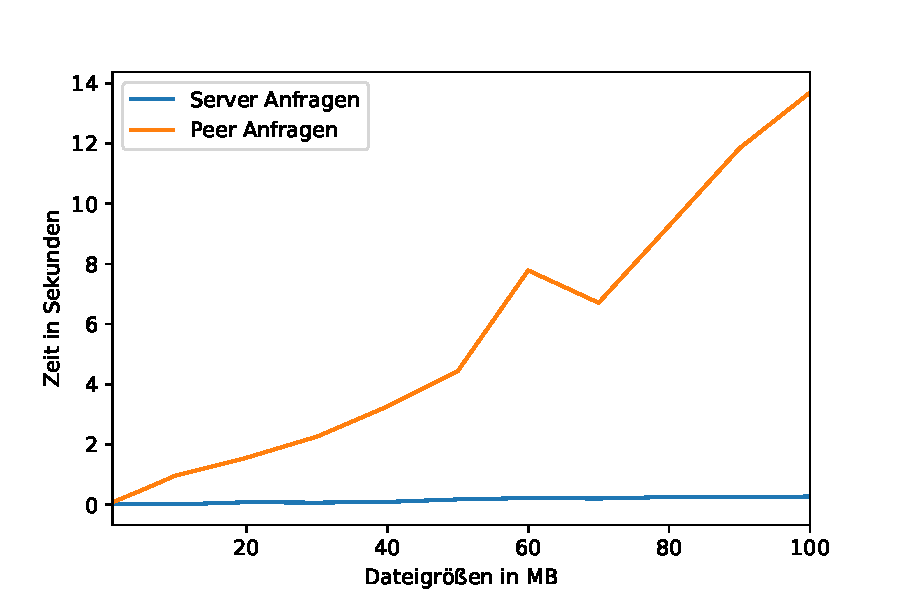
\includegraphics[width=0.8\textwidth]{figures/Timing_file_size}
	\caption[A Figure Short-Title]{}
	\label{fig:timing_file_size}
\end{figure}

\begin{figure}[!h]
	\centering
	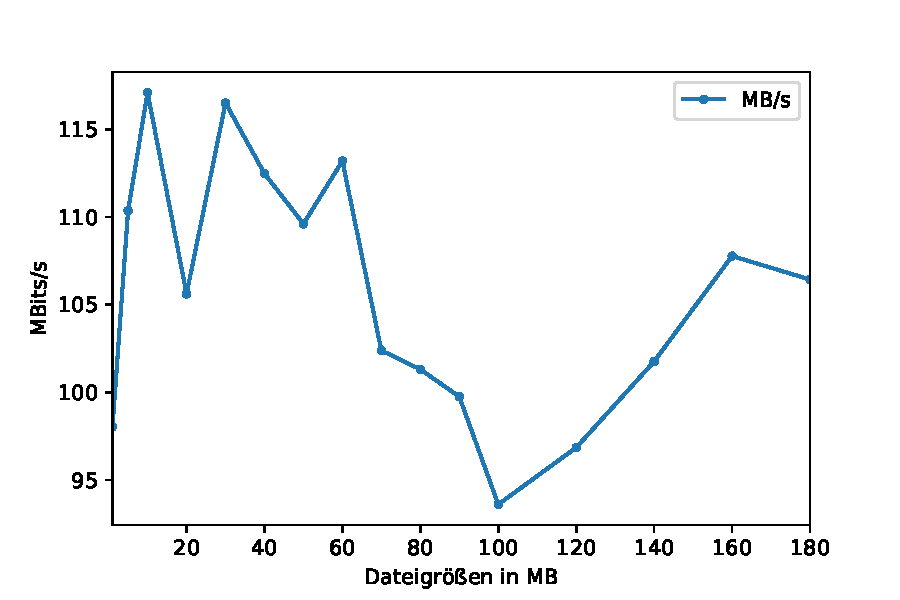
\includegraphics[width=0.8\textwidth]{figures/durchsatz_file_size}
	\caption[A Figure Short-Title]{Durchsatz}
	\label{fig:durchsatz_file_size}
\end{figure}


\begin{itemize}
	\item Mac book pro Ende 2013
	\item 2.3 ghz i7
	\item 16gb ram
	\item 1, 5, 10, 20, 30, 40, 50, 60, 70, 80, 90 , 100 mb
	\item durchsatz berechnen
	\item Limitierung durch websockets
	\item lokal auf einem Rechner um Netzlaufzeiten auszuklammern
	\item 1 Peer lädt vor
	\item der andere lädt von peer
	\item benchmarkt das nur das lokale netzwerk?? --> routingy
\end{itemize}
\subsection{Educational context}
\begin{itemize}
	\item machbarkeitstests in schule
	\item setup erklären
	
\end{itemize}

\subsection{Live Streaming}
\begin{figure}[!h]
	\centering
	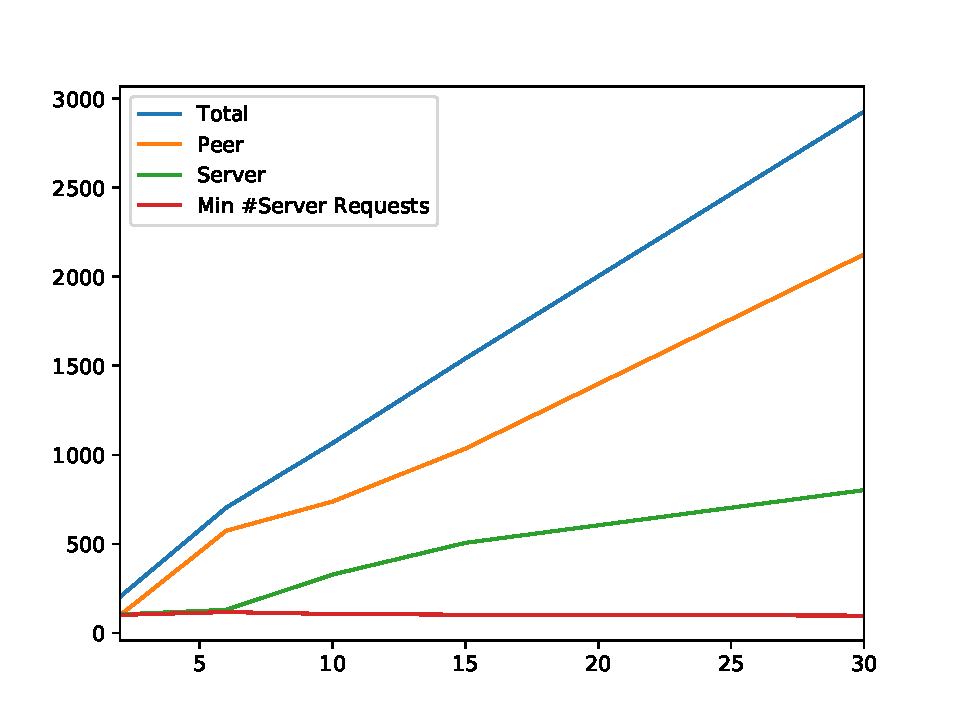
\includegraphics[width=0.8\textwidth]{figures/clients_line_chart}
	\caption[A Figure Short-Title]{Vergleich der Anfragen nach Anfrageart}
	\label{fig:live_stream_line_chart}
\end{figure}
Um die Funktionalität des \cdns im Falle eines Livestreams zu testen wurde ein Livestream mit der Infrastruktur von Slidesync aufgesetzt. Slidesync verwendet bei der Verteilung des Videos das Datenformat HLS. Das \cdn wurde so konfiguriert das ausschließlich die HLS Segmente über das \cdn behandelt werden. Sämtliche im folgenden betrachteten Anfragen sind demnach HLS Segmente. 

Der Test wurde in einem Unternehmensnetzwerk durchgeführt um die Funktionalität in einem solchen Netzwerk zu gewährleisten. In diesem Netzwerk wurden insgesamt 30 Rechner aufgestellt. Da es vor allem um den Durchsatz des \cdns ging wurde auf allen Clients ein aktueller Chrome Browser verwendet. Auf den Clients wurde zuerst die Event Seite geladen und erst im Anschluss der Livestream gestartet. Getestet wurden sechs, zehn, 15, 20 und 30 Clients, die sich alle im selben lokalen Netzwerk befanden. Der Streaming- und der Anwendungsserver befand sich außerhalb des Netzwerkes und waren nur über die Internetverbindung zu erreichen. Bei jedem Test wurde der Stream zehn Minuten laufen gelassen und alle Clients befanden sich in dem selben Peer Mesh.

\begin{figure}[!h]
	\centering
	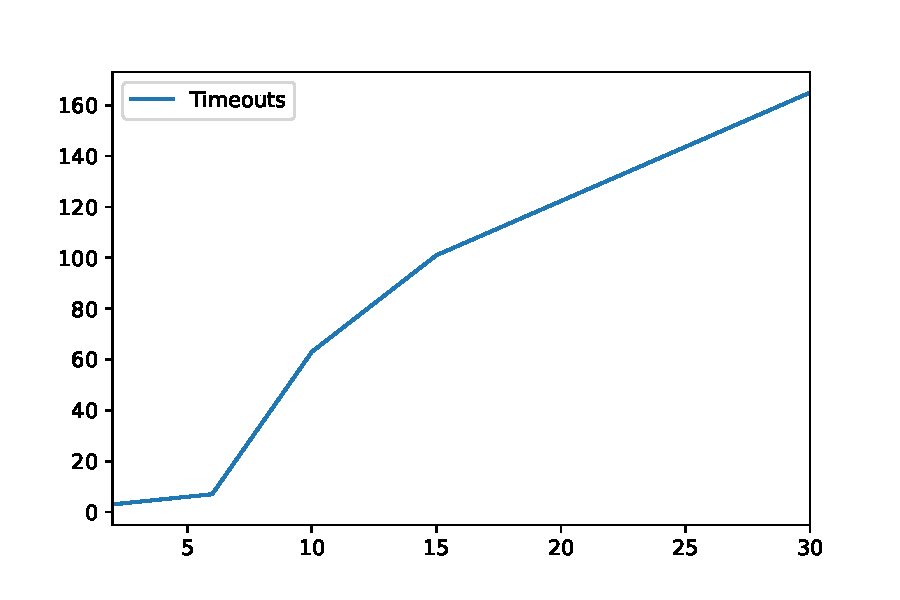
\includegraphics[width=0.8\textwidth]{figures/timeouts}
	\caption[A Figure Short-Title]{Anzahl der Timeouts des \cdns}
	\label{fig:timeouts}
\end{figure}


Abbildung \ref{fig:live_stream_line_chart} zeigt die Abhandlungsart der Anfragen. Dabei ist zu beachten das ca 100 Requests notwendig waren damit sämtliche HLS Segmente im \pTp Netzwerk verfügbar sind. Bei steigender Anzahl von Teilnehmern ist zu beobachten das eine größere Anzahl an Anfragen über den Server geladen werden müssen. Ein möglicher Grund hierfür ist Die Zeitliche Verteilung der Anfragen. Befinden sich mehr Peers im Netzwerk so wird es wahrscheinlicher das zwei Teilnehmer sich beide an der selben Stelle im Video befinden, die HLS Segmente laden müssen, jedoch noch kein Teilnehmer das Segment heruntergeladen hat. Auch wird es wahrscheinlicher das eine größere Anzahl an Teilnehmern ein Segment über den selben Teilnehmer laden wollen. Fragen zu viele Teilnehmer eine Ressource bei selben Teilnehmer an, so kann er nicht mehr alle Anfragen bearbeiten. Die Anfrage über das \pTp \cdn wird abgebrochen und über den Server geladen. Abbildung \ref{fig:timeouts} zeigt die Anzahl der Timeouts bei steigender Teilnehmerzahl. Dabei ist zu beachten das der Timeout so gewählt wurde das das Video weiterhin flüssig lief.

\begin{figure}[!h]
	\centering
	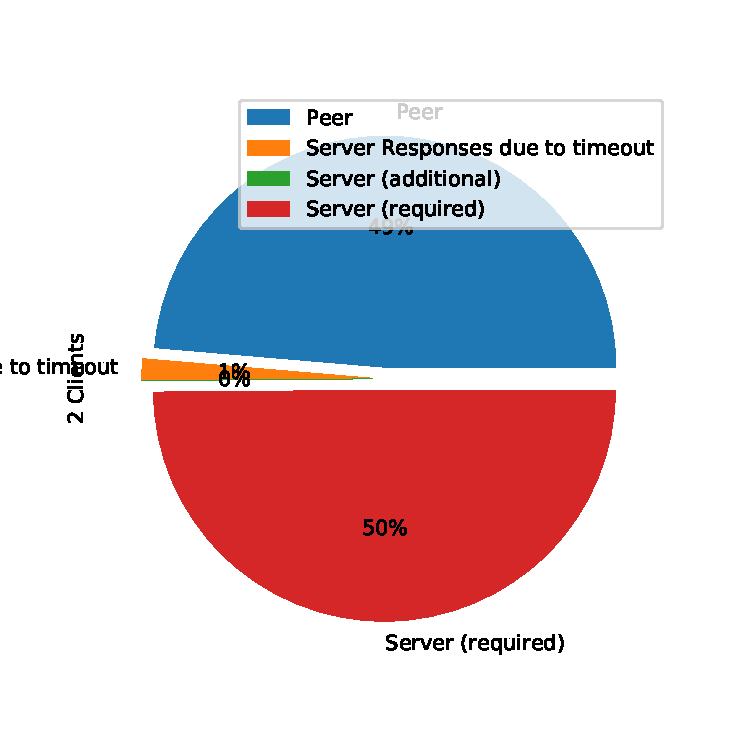
\includegraphics[width=0.45\textwidth]{figures/pie_2_clients}
	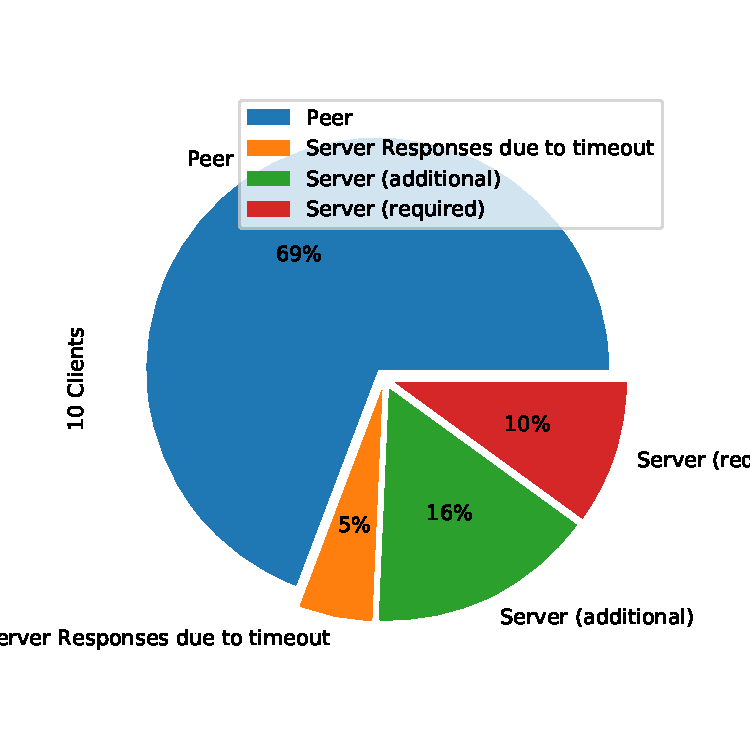
\includegraphics[width=0.45\textwidth]{figures/pie_10_clients}
	\caption[A Figure Short-Title]{Verteilung der Anfragen bei zwei und 10 Clients}
	\label{fig:corporate_pie_2}
\end{figure}
\begin{figure}[!h]
	\centering
	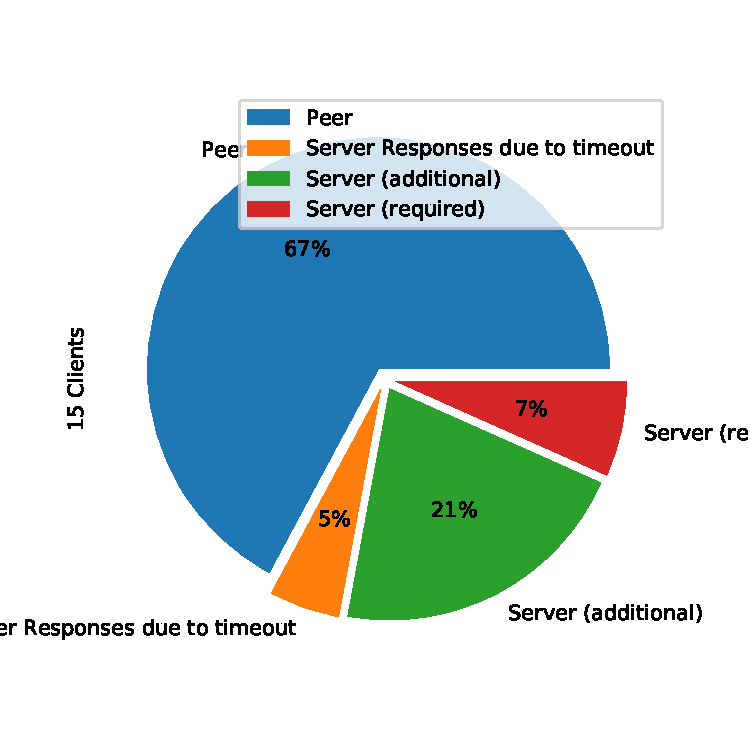
\includegraphics[width=0.45\textwidth]{figures/pie_15_clients}
	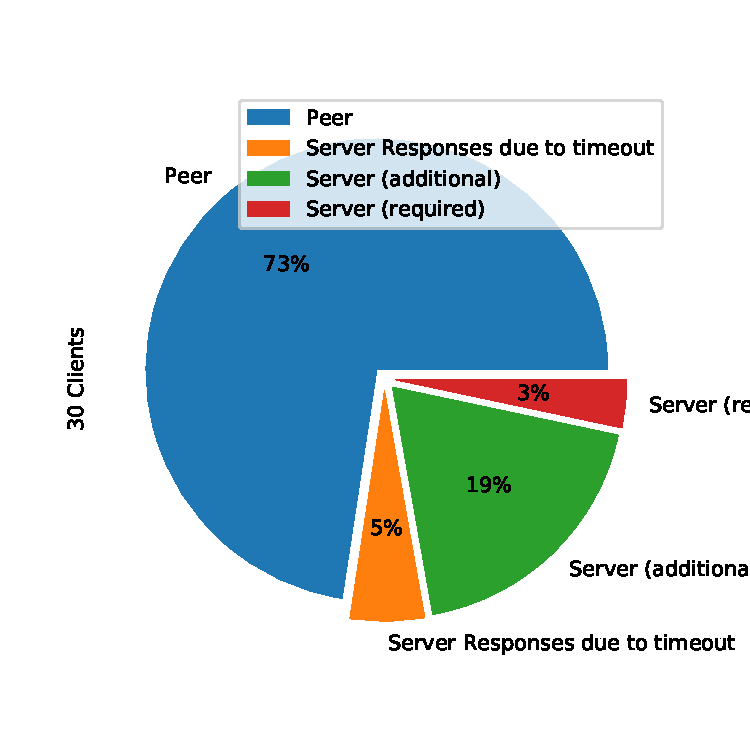
\includegraphics[width=0.45\textwidth]{figures/pie_30_clients}
	\caption[A Figure Short-Title]{Verteilung der Anfragen bei zwei und 10 Clients}
	\label{fig:corporate_pie_3}
\end{figure}

Betrachtet man die zusätzlich Notwendigen Server Anfragen so lässt sich beobachten das der Prozentsatz in diesem Test annähernd konstant ist.  

%\begin{figure}[!h]
%	\centering
%	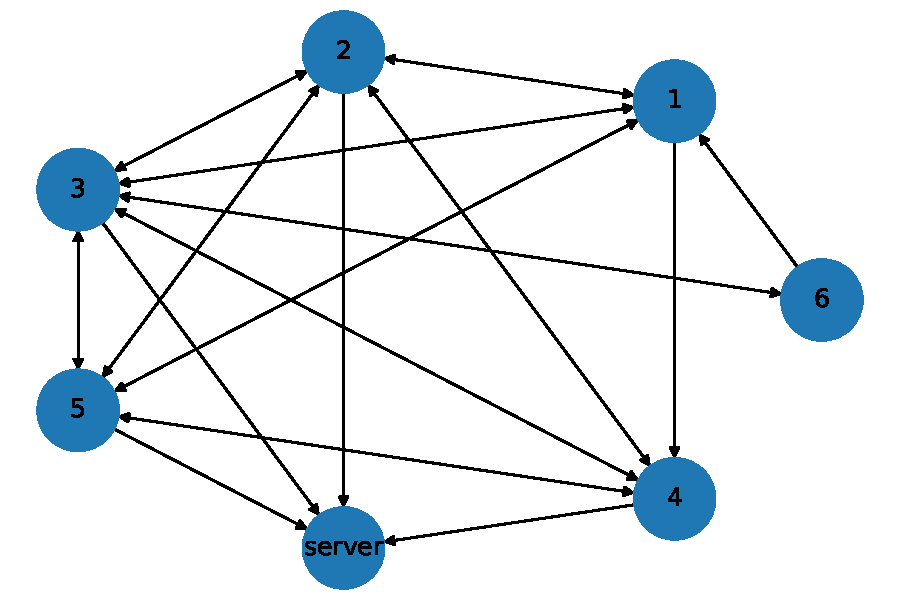
\includegraphics[width=0.8\textwidth]{figures/6_clients_network}
%	\caption[A Figure Short-Title]{Vergleich der Anfragen nach Anfrageart}
%	\label{fig:6_clients_network}
%\end{figure}

\begin{figure}[!h]
	\centering
	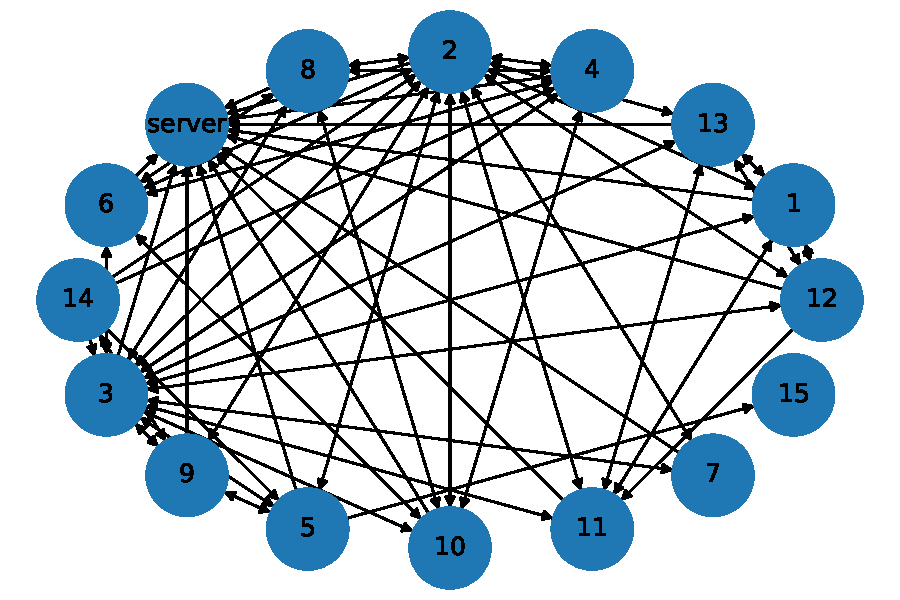
\includegraphics[width=0.8\textwidth]{figures/15_clients_network}
	\caption[A Figure Short-Title]{Vergleich der Anfragen nach Anfrageart}
	\label{fig:15_clients_network}
\end{figure}

Abbildung \ref{fig:15_clients_network} zeigt welche Teilnehmer untereinander Daten ausgetauscht haben. Auffällig ist das einige Teilnehmer besonders vielen Teilnehmern Daten gesendet haben. Dies war besonders dann der Fall wenn sie die einzigen im Netzwerk waren die das Segment bereits geladen hatten. Die meisten Kanten sind jedoch bidirektional, sprich zwar haben einige Teilnehmer besonders viele Anfragen beantwortet, jedoch haben sie sich nicht als zentrale Punkte des Netzwerkes etabliert sondern ebenfalls ihre Daten von anderen Teilnehmern geladen. \todo{gewichtung??} 

\begin{table}[!htb]
\begin{center}

	\begin{tabular}{|r|l|l|l|l|l|l|}
		\hline
		Request Art	 & #Anfragen 	& Durchschnitt 	& Standardbweichung	& Min		& Max	 \\ \hline
		Peer 		& 4571 				& 201.60	 ms	  	& 190.14	 ms				& 27.02 ms	& 2832.27 ms \\ \hline
		Server 		& 1870		 		& 63.61 ms		& 62.99	ms				& 9.41 ms	& 649 ms	\\
		\hline
	\end{tabular}
	\caption{Browser Storage Quotas }
\end{center}

\end{table}

Bei der Betrachtung der Ladezeiten wurden alle erfassten Anfragen berücksichtigt. Allerdings wurden die Daten um die Server Anfragen bereinigt bei denen zuvor das \pTp \cdn einen timeout verursacht hat. Insgesamt wurden 4571 Peer Anfragen und 1870 Server Anfragen betrachtet. 
Anfragen die vom \pTp \cdn beantwortet wurden brauchten im Durchschnitt 201,60ms. Server Anfragen waren im Vergleich mit 63,31ms im Durchschnitt deutlich schneller. Die ist auf den geringeren Durchsatz der \webrtc Datachannels zurückzuführen. (Siehe Dateigrößen \todo{ref}) Damit war das \pTp \cdn zwar deutlich langsamer, jedoch schnell genug um eine flüssige Wiedergabe zu gewährleisten. Da eine Anfrage die länger als 3000ms brauchte bei dem \pTp \cdn zu einem timeout geführt hat betrug die höchste erfasste Ladezeit 2832,27 ms.    
%\todo{einige clients haben keine daten an den server gesendet. Rausrechnen!}
%\begin{itemize}
%	\item ladezeiten
%	\item Alle Anfragen berücksichtigt
%	\item 4571.0 peerRequest
%	\item serverResponse   1870.0
%	\item Serveranfragen bereinigt um die Timeouts
%\end{itemize}
\subsection{Nutzerzufriedenheit}
wie soll das aussehen?

\section{Security considerations}
\section{DRM licencing}
%passt hier nicht wirklich hin